%************************************************
\chapter{Andamento do projeto}\label{ch:introducao}
%************************************************
\section{Sumário do projeto inicial}
Neste projeto, propomos o desenvolvimento de um método de reconhecimento de enovelamentos proteicos utilizando autômatos celulares. O reconhecimento do enovelamento é uma etapa crucial para expandir a utilização da modelagem comparativa, pois permite identificar proteínas que tenham estruturas semelhantes, mesmo na ausência de alta similaridade entre suas estruturas primárias. Além do reconhecimento do enovelamento proteico, os autômatos celulares apresentam características que os tornam capazes de fornecer também informações sobre a dinâmica do enovelamento, sendo, portanto, um método promissor nesta área, mas até então inédito.

Autômatos celulares são modelos computacionais que consistem num conjunto de células discretas espacialmente, as quais encontram-se em estado discreto num tempo também discreto. O estado dessas células podem se alterar ao longo do tempo para outros estados discretos pertencentes à um conjunto finito de estados possíveis. A alteração desses estados ao longo do tempo é chamada de evolução, e é definida por regras de transição simples e locais, onde o estado atual da célula e de seus vizinhos definirá para qual estado a célula irá evoluir. Esta evolução, muitas vezes, produz padrões complexos a partir do efeito cooperativo desses elementos simples - as regras e as células. Essa complexidade que surge globalmente no sistema a partir de regras simples, locais e determinísticas é conhecida como Emergência. A figura \ref{fig:ca} exemplifica um autômato celular elementar. 

\begin{figure}[h]
	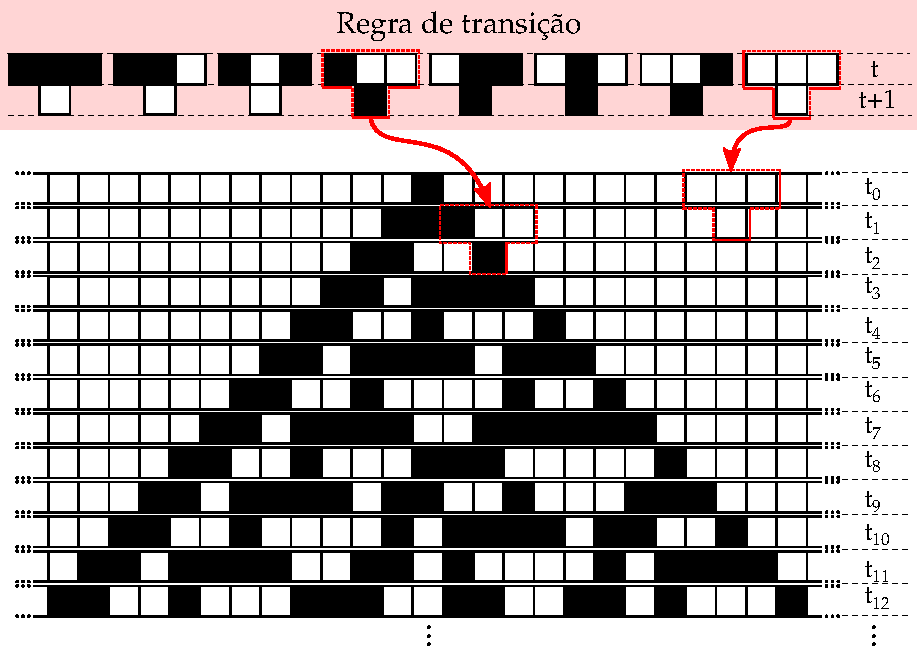
\includegraphics[width=1\linewidth]{ca_final}
	\caption{Exemplo de um autômato celular elementar. Este é o tipo de autômato celular mais simples, pois é unidimensional, possui apenas dois estados (0 ou 1) e possui vizinhança 1 (uma célula a esquerda e uma a direita). O autômato inicia com uma linha de células ($t_{0}$) e evolui através da aplicação de uma regra de transição que irá determinar o estado de cada uma das células na geração seguinte ($t_{1}$). Este processo ocorre iterativamente produzindo, muitas vezes, uma complexidade global que emerge da aplicação das regras de transição locais.}
	\label{fig:ca}
\end{figure}

Visando o objetivo principal de desenvolver um método de reconhecimento de enovelamentos proteicos baseado em autômato celulares foram estipuladas algumas etapas de menor complexidade e custo computacional. Essas etapas permitirão avaliar progressivamente o potencial do método e assim direcionar o desenvolvimento e contornar possíveis dificuldades.

Uma dessas etapas é a utilização de autômatos celulares para a predição de estruturas secundárias proteicas. As estruturas secundárias são estruturas locais e acredita-se que durante o enovelamento elas se originam em determinadas regiões da sequência de aminoácidos e propagam-se, formando uma estrutura secundária semelhante a encontrada na proteína em sua conformação nativa. Essa característica de iniciar localmente e propagar-se formando a estrutura secundária sugere que este é evento promissor para ser modelado por autômatos celulares. A figura \ref{fig:ca_ss} representa um modelo de autômato celular unidimensional aplicado a predição de estruturas secundárias proteicas.

\begin{figure}[h]
	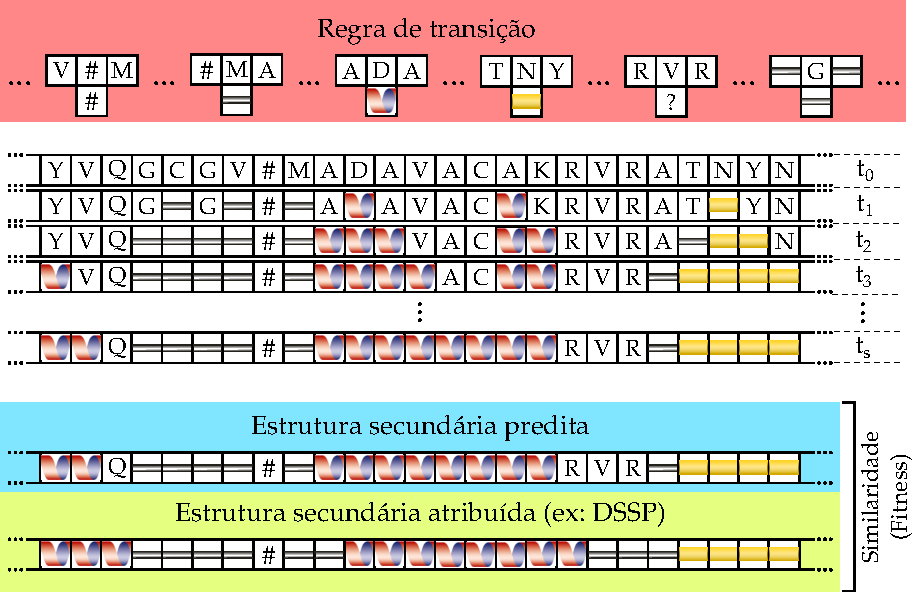
\includegraphics[width=1\linewidth]{ca-ss_final}
	\caption{Esquema de um autômato celular para a predição de estruturas secundárias. A regra de transição do autômato é composta de 13824 elementos. O estado inicial do autômato ($t_{0}$) é formado pela sequência de aminoácidos da proteína. O estado $\#$ indica o início ou fim da cadeia polipeptídica e pode ser utilizado para concatenar múltiplas proteínas, funcionando como uma barreira de influência entre elas. O estado final do autômato celular $t_{n}$, onde $n$ é um número finito, é a estrutura secundária predita e sua similaridade com a estrutura secundária atribuída pode ser considerada uma medida do acurácia da regra de transição.}
	\label{fig:ca_ss}
\end{figure}

No entanto, a principal dificuldade do projeto consiste em encontrar regras de transição para os autômatos celulares capazes de reproduzir o evento desejado. Essa dificuldade ocorre devido ao imenso espaço de regras possíveis. Por exemplo, considerando apenas regras que contenham os estados correspondentes aos aminoácidos e a elementos de estrutura secundária, como na figura \ref{fig:ca_ss}, teríamos $4^13225$ combinações, ou regras, possíveis que poderiam predizer a formação de estrutura secundária a partir da sequência de aminoácidos.


\section{Análise do período}
Neste período, o código fonte inicial foi quase totalmente refeito para permitir maior flexibilidade. Isso foi necessário, pois o código desenvolvido inicialmente e que foi utilizado em testes preliminares, abrangia apenas a predição da estruturas secundárias das proteínas e tinha como objetivo avaliar a viabilidade do projeto. 

As modificações feitas no código permitirão criar autômatos celulares com outros estados além dos já utilizados, que correspondem aos aminoácidos e  elementos de estrutura secundária. Isso possibilitará testarmos tanto códigos simplificados que representem, por exemplo, as características físico-químicas dos aminoácidos, como carga, polaridade, entre outros, assim como códigos mais complexos que representem, por exemplo, diversos elementos de estrutura secundária juntamente com a exposição ao solvente.

\begin{figure}[h]
	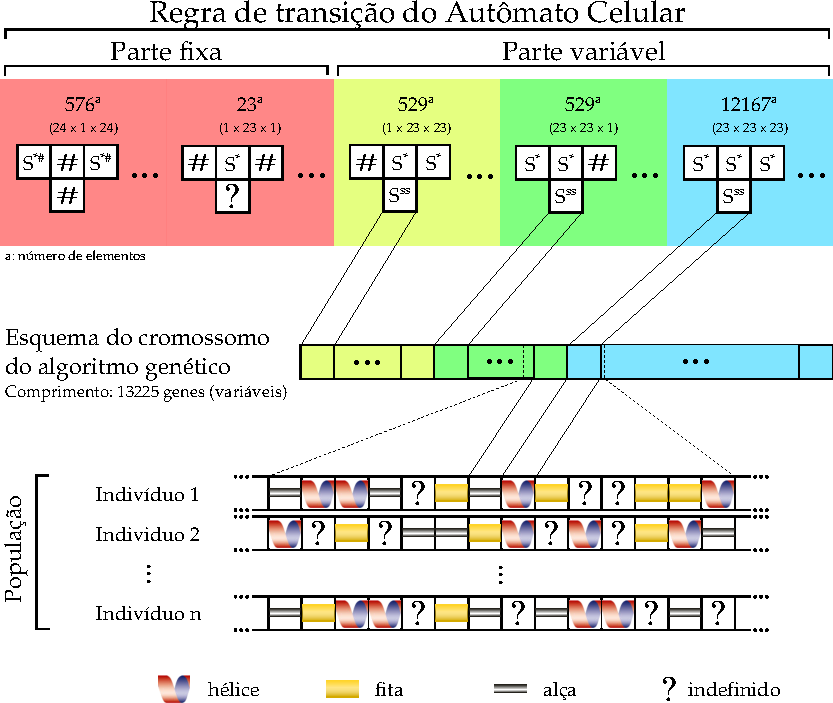
\includegraphics[width=1\linewidth]{ca_ga_final}
	\caption{Representação da utilização de um algoritmo genético na busca por uma regra de transição capaz de predizer estrututuras secundárias proteicas. Os cromossomos possuem 13225 genes, ou variáveis, que podem assumir quatro estados distintos. Cada indivíduo apresenta uma combinação desses estados. Essa combinação corresponde a uma regra de transição de um autômato celular que irá evoluir por um número definido de passos. A comparação do resultado dessa evolução com a estrutura secundária atribuída ("real") fornece uma medida do fitness da regra. Utilizando-se um algoritmo genético competente esperasse que ocorra uma convergência para a regra com maior fitness, ou seja, a que melhor prediz a estrutura secundária da proteína.}
		\label{fig:ca_ga}
\end{figure}

Diversos 



Com a modificação dos objetivos do projeto para a criação de um método de reconhecimento de enovelamentos proteicos
\section{Discussões e conclusões parciais}
Discussões 
\section{Perspectivas futuras}
No próximo periodo
